\begin{Exercise}[title=Résistances équivalentes]
  \ExePart Calculer la résistance équivalent de ce réseau ( chaque
  coté possède une résistance $R$) entre: \Question A et C, A et E , A
  et F \Question B et D, A et B , B et F
  \begin{center}
    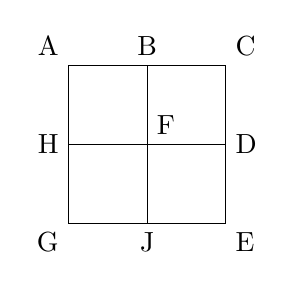
\begin{tikzpicture}
      \draw (0,0)node[below left]{G} -- (0,2)node[above left]{A};
      \draw (0,0) -- (2,0)node[below right]{E}; \draw (2,0) --
      (2,2)node[above right]{C}; \draw (0,2)-- (2,2); \draw
      (0,1)node[left]{H} --(2,1)node[right]{D}; \draw
      (1,0)node[below]{J} -- (1,2)node[above]{B}; \draw
      (1,1)node[above right]{F};
    \end{tikzpicture}
  \end{center}
  \ExePart Calculer la résistance équivalent de ce réseau à maille
  carré entre A et B
  \begin{center}
    \begin{tikzpicture}
      \draw (0,0)node[below left]{A} grid (3,3)node[above right]{B};
    \end{tikzpicture}
  \end{center}
  \ExePart
  \begin{center}
    \begin{circuitikz}
      \draw (-0.5,0) --(0,0)node[above left]{A} -- (0,1) to[R,l=$R_1$]
      (2,1)node[above]{C} to[R,l=$R_2$](4,1) -- (4,0)node[above
      right]{B}--(4.5,0); \draw (-0.5,0) --(0,0) -- (0,-1)
      to[R,l=$R_2$] (2,-1)node[below]{D} to[R,l=$R_1$](4,-1) -- (4,0);
      \draw (2,-1) to[R,l=$R$] (2,1);
    \end{circuitikz}
  \end{center}
  \Question Calculer la résistance équivalente entre A et B.
  \Question On applique entre A et B $U=11V$ calculer $i_{CD}$ avec
  :$R_1=2R$, $R_2=4R$, $R= 1\Omega$.
\end{Exercise}
\begin{Answer}
  \ExePart
Replier sur la diagonale les points d'équipotentiels.
  $R_{eq}=\frac{13}{7}R$\\
  \ExePart \Question $5R/4$, $3R/2$ $7R/8$ \Question $5R/6$, $R$,
  $7R/12$
  \ExePart \Question
  On a :
  \[
    \begin{cases}
      u = u_2'-u_c+u_2 = u_1'+u_c+u_1\\
      i = i_1+i_2 = i_1'+i_2' \\
      i_c = i_1'-i_2  \\
    \end{cases}
    \implies
    \begin{cases}
      2u = R_1(i+i_c)+R_2(i-i_c)\\
      0 = 2Ri_c +R_1(i+i_c)-R_2(i-i_c)\\
      i+i_c = i_1+i_1'\\
      2 i = i_1+i_1'+i_2+i_2'
    \end{cases}
  \]
  Donc :
  \[
    \begin{cases}
      i_c  = \frac{R_2-R_1}{2R+R_1+R_2}i  = a i \\
      2 u = R_1(1+a)i+R_2(1-a)i
    \end{cases}
\]
Donc:
\[R_{eq}=\frac{2R_1R_2+RR_1+RR_2}{2R+R_1+R_2}\]
\Question $I=1 A $
\end{Answer}
